\documentclass[17pt, t, lualatex]{beamer}



\title{Hidrodinámica del Río Magdalena a la altura de Barrancabermeja: Limpieza de datos, modelo y despliegue}
\date{\today}
\institute[UJTL]{Universidad Jorge Tadeo Lozano}
\author{Ludwig Alvarado Becerra}

\usepackage{amsmath, amssymb, mathtools}
\usepackage[spanish]{babel}
\usepackage{biblatex}
\usepackage{hyperref}
\usepackage{xurl}
\usepackage{svg}
\usepackage{listings}
\usepackage[scale=7]{ccicons}


\addbibresource{referencias.bib}  % Make sure your .bib file is correctly named


\addbibresource{referencias.bib}


\definecolor{white}{HTML}{FFFFFF}
\definecolor{sand}{HTML}{EBE5E0}
\definecolor{KTHblue}{HTML}{004791}
\definecolor{skyblue}{HTML}{6298D2}
\definecolor{navy}{HTML}{000061}
\definecolor{lightblue}{HTML}{DEF0FF}
\definecolor{digitalblue}{HTML}{0029ED}


\lstset{
  language=bash,                       % Set the language to bash
  backgroundcolor=\color{white},       % Background color for the code block
  basicstyle=\ttfamily\normalsize,    % Use typewriter font and small size
  keywordstyle=\color{KTHblue},           % Style for keywords (e.g. if, for, etc.)
  commentstyle=\color{sand},          % Style for comments
  stringstyle=\color{skyblue},             % Style for strings
  showstringspaces=false,              % Don't underline spaces in strings
  breaklines=true,                     % Automatically break long lines
  frame=single,                        % Add a frame around the code
  captionpos=b,                        % Position of the caption (bottom)
  numbers=left,                        % Line numbers on the left
  numberstyle=\tiny\color{gray},       % Style for line numbers
  stepnumber=1,                        % Display every line number
  numbersep=5pt,                       % Space between line numbers and code
  morekeywords={bat, wc, tail, cut, head, >},
}



% Probably load as late as possible
% Other options are
% - engine=pdflatex to compile in pdfLaTeX (with different fonts),
% - mathshape=rm to use serif font for math,
% - mathsahpe=custom to not set any math font (so that you can define your own math fonts)
\usetheme[engine=lualatex, mathshape=sf, fontdir=kthpq-files/fonts/Figtree/]{kthpq}
\setmonofont{Bitstream Vera Sans Mono}[Scale=.9]

% Custom colors (see beamercolorthemecustom.sty for more details)
% \usecolortheme{custom}

% Modify the headline template: KTH-full, KTH-section-only, or KTH-frametitle-only.
% \setbeamertemplate{headline}[KTH-full]

% Custom footline
% \setfootline{left}{center}{right}



\begin{document}

\inserttitlepage

\section{Recapitulación}

\insertsectionpage

\begin{frame}[allowframebreaks]
  \frametitle{Recapitulación}

  \begin{itemize}
    \item \textbf{Se tiene:}
          \begin{itemize}
            \item Coeficiente de rugosidad de Manning\cite{garcia2020mathematical}. 
            \item Dimensiones del río de ancho y largo.
            \item Pendiente del río.
          \end{itemize}
    \item \textbf{Falta:}
          \begin{itemize}
            \item Limpieza de duplicados con los datos de la elevación del río.
            \item Limpieza general de datos del caudal del río.
            \item Condiciones iniciales y finales.
            \item Implementación en código del modelo.
          \end{itemize}
  \end{itemize}

\end{frame}

\section{Limpieza de datos}

\insertsectionpage

\begin{frame}[allowframebreaks]
  \frametitle{Limpieza datos de elevación del río}
      \begin{itemize}
        \item Según Cormagdalena\cite{cormagdalena_niveles} se registran niveles de la elevación en los últimos $~200$ días.
        \item Al realizar \lstinline|bat niveles.csv \| wc -l| da una salida de $1801$.
        \item Utilizando de la librería \textit{Pandas} y \textit{Python} se realiza una limpieza de duplicados y también una conversión de \textit{data type} a \textit{datetime}.
      \end{itemize}

      \newpage

      \begin{figure}[ht]
        \centering
        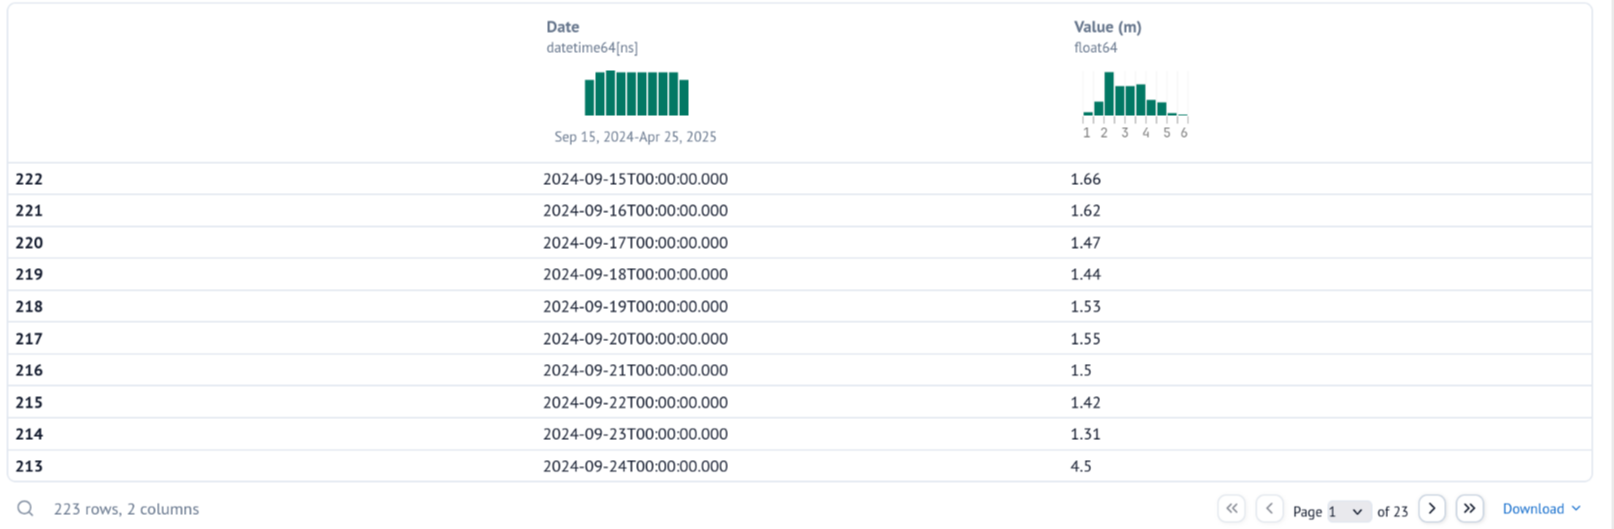
\includegraphics[width=\textwidth]{img/img1.png}
        \caption{Resultado de una celda en \textit{Marimo}, elaboración propia.}
      \end{figure}

\end{frame}

\begin{frame}[allowframebreaks]
  \frametitle{Limpieza datos del caudal}
\begin{columns}
  \begin{column}{.5\textwidth}
    \begin{itemize}
      \item Datos descargados del GRDC\cite{grdc_data_portal} y propiedad del Instituto de Hidrología, Metereología y Estudios Ambientales (IDEAM)\cite{ideam2025}.
      \item Datos desde enero de $1936$ hasta septiembre de $2024$.
      \item Formato ``YYYY-MM-DD;hh:mm; Value''.
    \end{itemize}
  \end{column}

  \begin{column}{.5\textwidth}
    \begin{figure}[ht]
      \centering
      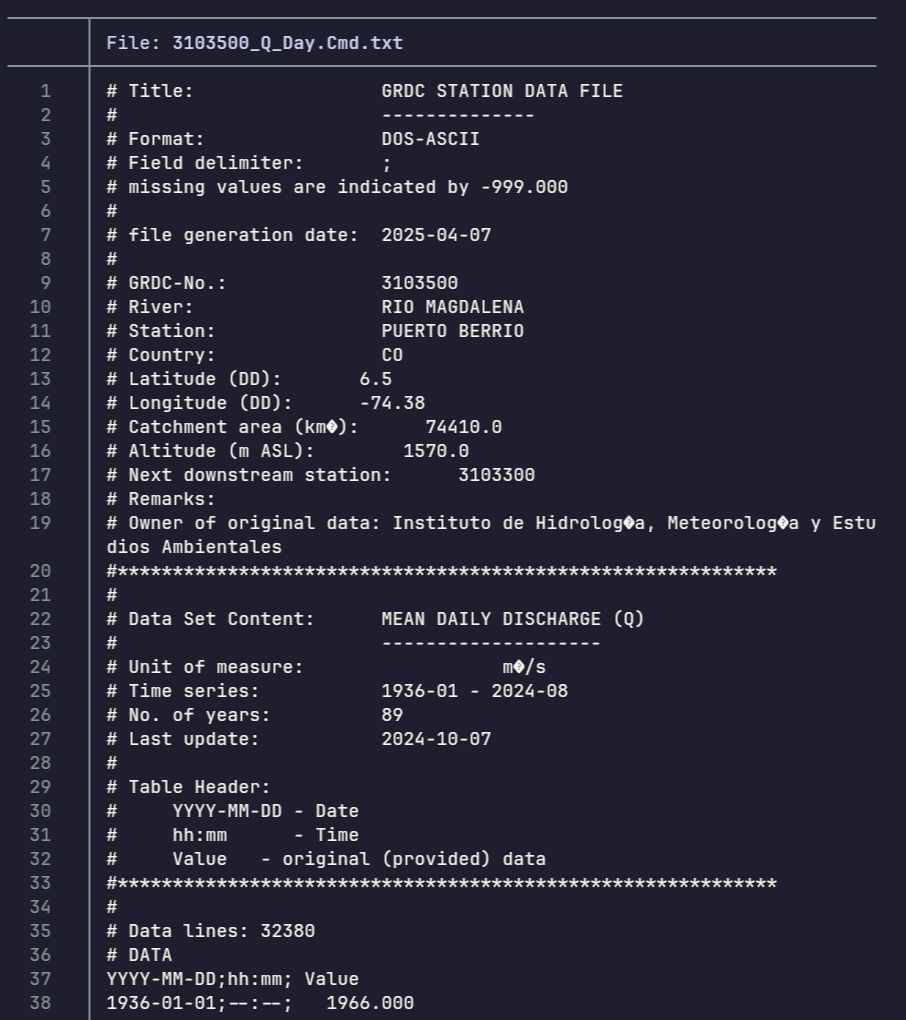
\includegraphics[width=0.6\textwidth]{img/img2.png}
    \end{figure}
  \end{column}

\end{columns}

\newpage

\begin{columns}
  \begin{column}{.5\textwidth}
    \begin{itemize}
      \item Se utiliza la funcionalidad de \textit{pipelines} en UNIX para filtrar los datos.
      \item Se ejecuta \lstinline|tail -n +37 3103500_Q_Day.Cmd.txt \| cut -d ";" -f 1,3 \| head|
      \item Finalmente, se ejecuta \lstinline|tail -n +37 3103500_Q_Day.Cmd.txt \| cut -d ";" -f 1, 3 > Caudal.txt|
    \end{itemize}
  \end{column}

  \begin{column}{.5\textwidth}
    \begin{figure}[ht]
      \centering
      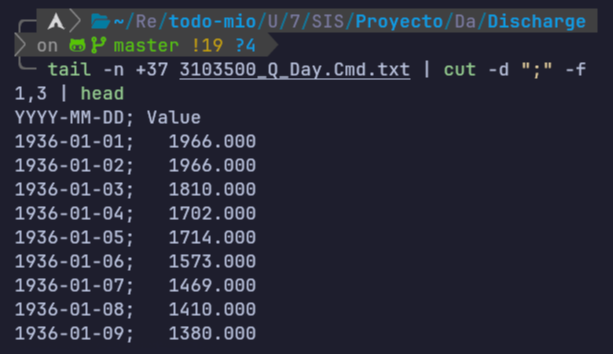
\includegraphics[width=\textwidth]{img/img3.png}
    \end{figure}

  \end{column}
\end{columns}

\newpage

\begin{columns}
  \begin{column}{.5\textwidth}
    \begin{itemize}
      \item Último dato registrado del caudal: $2024-08-25$.
      \item Primer dato registrado de la elevación del río: $2024-09-15$.
      \item Se toman períodos con variabilidad climática similar.
    \end{itemize}
  \end{column}

  \begin{column}{.5\textwidth}
\begin{figure}[ht]
  \centering
  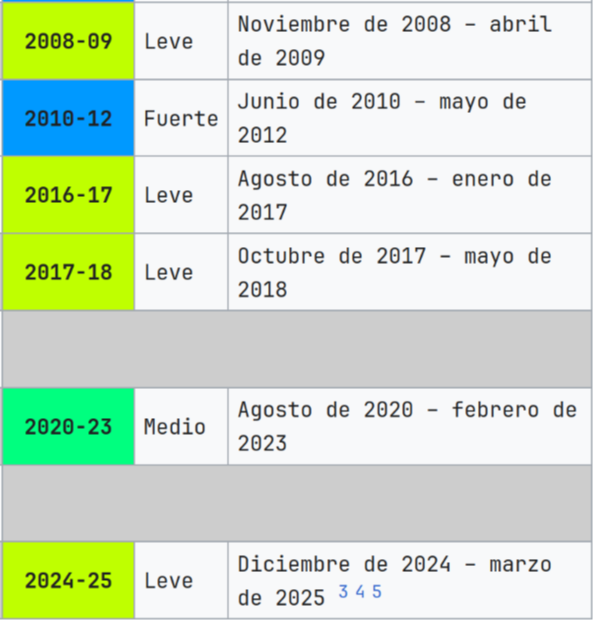
\includegraphics[width=0.5\textwidth]{img/img4.png}
  \caption{Sacado de \textit{Anexo:Eventos de El Niño y La Niña en el siglo XXI}\cite{eswiki:166933650}.}
\end{figure}

  \end{column}
\end{columns}

\newpage 

\begin{figure}[ht]
  \centering
  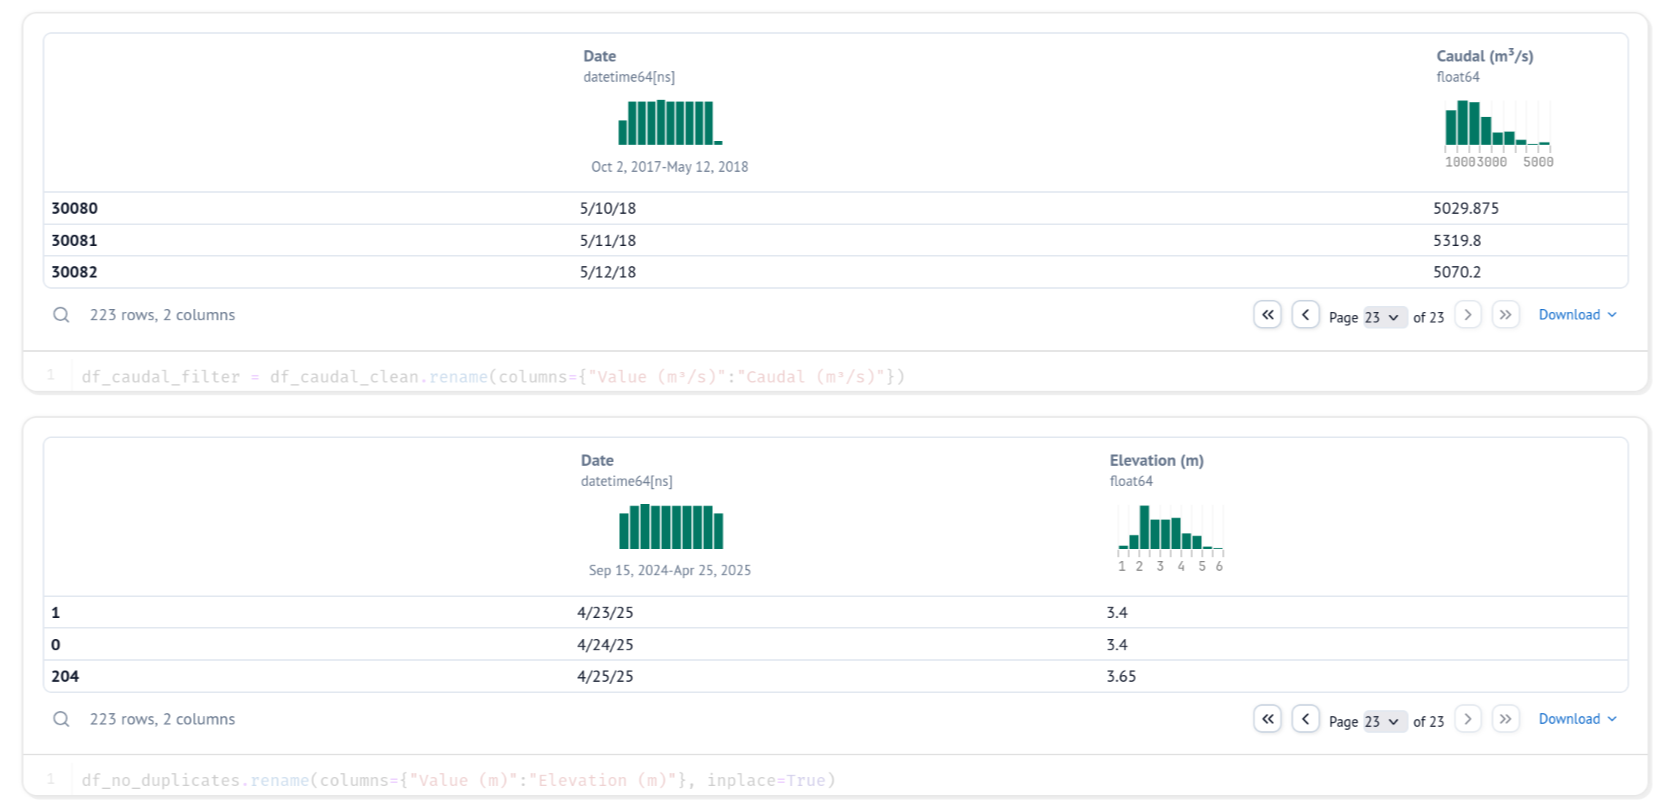
\includegraphics[width=0.7\textwidth]{img/img5.png}
  \caption{Datos del caudal filtrados desde el 1 de octubre de 2017 y el 12 de mayo de 2018. El \textit{dataset} de la altura está completo. Elavoración propia usando \textit{Marimo}.}
\end{figure}




\end{frame}








\begin{frame}
  \frametitle{Licencia}

  \begin{columns}
    \begin{column}{.5\textwidth}
      \begin{itemize}
        \item Código, datos y contenido se encuentra en: \url{https://github.com/TheLudway/HydrologyDynamicsProject} 
        \item Todo bajo la licencia GPL V3 y CC BY SA 4.0 a excepción de los datos.
      \end{itemize}
    \end{column}

    \begin{column}{.5\textwidth}
      \begin{figure}[ht]
        \centering
        \href{https://www.gnu.org/licenses/gpl-3.0.txt}{\includesvg[width=0.8\textwidth]{img/GPL.svg}}
      \end{figure}
    \end{column}
  \end{columns}

\end{frame}


\section{Referencias}

\insertsectionpage
\begin{frame}[allowframebreaks]{Referencias}
  \printbibliography
\end{frame}


\insertendpage

\end{document}
